\chapter{Optimizing patients travel}

\section{Context}

% TODO

% Early diagnosis importance
In breast cancer, early detection, diagnosis and initiation of treatment within 90 days increase survival \cite{williams_assessment_2015}.
Patient and system delays of 6 months were significantly associated with more advanced-stage disease \cite{pace_delays_2015}.
Delay in seeking medical attention for breast cancer symptoms, as well as delay in the diagnosing of and delivery of effective treatments for breast cancer may result in advanced states of disease, thereby contributing to breast cancer mortality \cite{caplan_delay_1992}.

% Role of \ac{gp} in Healthcare
GPs play a crucial role in early cancer detection because the majority of cancer patients initially consult their \ac{gp} with symptoms. In approximately 50\% of patients who begin the diagnostic journey in general practice, the \ac{gp} will suspect cancer at the first presentation, and the suspicion is more often raised when the patient present with alarm symptoms. The \ac{gp} often has a range of strategies available for further relevant diagnostics including in-house options as ``wait-and-see'', blood tests and medical treatment such as prescription medicine. The \ac{gp} can also act as a gatekeeper to e.g. specialized private practices, Cancer Patient Pathways (CPP) or diagnostic imaging (e.g. CT scan). Therefore, the actions taken by the \ac{gp} upon the patient's symptom presentation may considerably affect the cancer trajectory. Nevertheless, it is unknown if the \ac{gp}'s diagnostic strategy is affected by the patient's travel distance to the medical facility performing cancer diagnostic investigations \cite{flytkjaer_virgilsen_cancer_2019}.

% Impact of travel on patients
We produce maps of travel time with and without access to motorized transport, thus characterizing travel time to healthcare for populations distributed across the wealth spectrum. We find that just 8.9\% of the global population (646 million people) cannot reach healthcare within one hour if they have access to motorized transport \cite{weiss_global_2020}.

There is great debate on whether centralized care actually improves survival and morbidity. A centralized approach often involves patients travelling relatively far away from their local community hospitals, and the social impact on patient wellbeing needs to be justified by evidence of improved care and better outcomes \cite{woo_centralisation_2012}.

However, there are also drawbacks to increasing the distance some patients travel to receive treatment. A number of authors have documented the distance decay association, which identifies that those who live closer to healthcare facilities have higher rates of usage after adjustment for need than those who live further away. In the debate between local versus centralized healthcare provision, 77\% of the included studies showed evidence of an association between worse health outcomes the further a patient lived from the healthcare facilities they needed to attend. This was evident at all levels of geography—local level, interurban and intercounty level. A distance decay effect cannot be ruled out, and distance/travel time should be a consideration when configuring the locations of healthcare facilities and treatment options for patients \cite{kelly_are_2016}.

Renal dialysis is a lifesaving but demanding therapy, requiring 3 weekly treatments of multiple-hour durations. Median travel distance was 4 times that in rural (10.9 miles) versus urban areas (2.6 miles). Most dialysis patients have higher rated facilities located not much further than their closest facility, suggesting many patients could evaluate tradeoffs between distance and quality of care in where they receive dialysis. Our results show that such tradeoffs likely occur \cite{salerno_understanding_2022}.

This literature review aims to identify the impact of travel on cancer patients' experiences of treatment. With centralization of cancer services, patients may have to travel considerable distances from their homes and families, to receive specialist cancer treatment. Centralization of cancer services may have advantages in terms of concentrating clinical expertise, enhancing the range of ancillary facilities and rationalizing the provision of expensive specialist equipment, but it is not known to what extent patients are affected by additional travel and the prospect of separation from their social networks. Travel to cancer treatment is described as inconvenient and a practical hardship for many patients and may be perceived, or experienced as, a barrier to treatment for some \cite{payne_impact_2000}.

Longer travel distance between the residence of the patient and the diagnosing hospital was associated with longer diagnostic intervals. This association was primarily driven by cancer patients diagnosed with cancer types that were hard to diagnose \cite{flytkjaer_virgilsen_cancer_2019}.

For most of the easy-to-diagnose cancer types (rectum cancer, malignant melanoma and testis cancer), a longer distance to the hospital was associated with increased odds of advanced tumour stage at diagnosis. For stomach, pancreatic, lung and ovarian cancer (i.e., the hard to diagnose cancer types), there was a consistent pattern where longer travel distance to the hospital was associated with decreasing odds of advanced disease stage \cite{virgilsen_travel_2019}.

In almost all the studies analyzed, patients who lived far from hospitals and had to travel more than 50 miles had a more advanced stage at diagnosis, lower adherence to encoded treatments, a worse prognosis, and a worse QoL \cite{ambroggi_distance_2015}.

Travel burden influences treatment compliance, as reported in two studies
\cite{dutta_evaluation_2013,guidry_transportation_1997}.

The distance from the hospital (i.e., travel burden) also influences the choice of appropriate treatment by cancer patients. Some studies found that patients living farther from a radiation treatment facility more often underwent mastectomy instead of BCS \cite{schroen_impact_2005,celaya_travel_2006,voti_treatment_2006,meden_relationship_2002,nattinger_relationship_2001,boscoe_geographic_2011} or did not undergo radiotherapy after BCS \cite{satasivam_dilemma_2014,schroen_impact_2005,celaya_travel_2006}. The results reported by Schroen et al. \cite{schroen_impact_2005} suggest that a marked change in geographic access to radiotherapy by opening new facilities might correlate with an increase in the proportion of patients undergoing breast conservation therapy. Tracey et al. \cite{tracey_patients_2015} found that patients with localized NSCLC were most likely to not undergo potentially curative surgery if they lived far from a specialist hospital and only attended a general hospital for their care.

% Importance of hospital routing
These barriers were more commonly perceived among patients who were younger, had lower socioeconomic status, and lived outside of Mexico City. The diagnosis interval was longer among those who used several different health services prior to the cancer hospital and perceived medical errors in these services. More health services were used among those who perceived errors and long waiting times for appointments, and who first consulted private services. Our findings support the relevance of strengthening early cancer diagnosis strategies, especially the improvement of quality of primary care and expedited referral routes to cancer services \cite{unger-saldana_barriers_2018}.

The necessity for repeated visits for cancer diagnosis and treatment on an outpatient or an inpatient basis makes distance an important issue with which the patient with cancer must manage during the disease course \cite{guidry_transportation_1997}.

In Rwanda, a low level of education and seeing a traditional healer first were significantly associated with a longer patient delay. Having made 5 health facility visits before the diagnosis was significantly associated with a longer system delay. However, being from the same district as one of the two hospitals was associated with a decreased likelihood of system delay \cite{pace_delays_2015}.

Contacting a provincial hospital instead of a university hospital as first medical care, being given a diagnosis rather than being told nothing and being given treatment rather than being immediately referred were associated with system delay. System delay in hospitals outside the university needs to be improved by a good referral system \cite{thongsuksai_delay_2000}.

The hazard of death from ovarian cancer was greater in women treated at a public general hospital than in women treated at a gynecological oncology service (GOS) \cite{tracey_effects_2014}.

Patients living farther from a radiotherapy service were more likely to die of rectal cancer, with 6\% increase in mortality risk found for each 100km increase in distance from the nearest radiotherapy facility \cite{baade_distance_2011}.

% Living in rural areas
Rural cancer patients face many challenges in receiving care, including limited availability of cancer treatments and cancer support providers (oncologists, social workers, mental healthcare providers, palliative care specialists, etc), transportation barriers, financial issues, and limited access to clinical trials \cite{charlton_challenges_2015}.

A general pattern of poorer survival and variations in clinical management for Australian female patients with breast cancer from non-metropolitan areas was evident \cite{dasgupta_variations_2018}.

Women resident in rural areas tended to receive less BCS than those from metropolitan areas. Women treated in a rural hospital had a reduced likelihood of BCS \cite{hall_unequal_2004}.

By focusing on patients' experience of vulnerability, this study corroborates previous knowledge and concerns related to health care access in rural and remote areas (such as distance, transportation, weather conditions, shortage of health care professionals, and limited availability of health care services), highlighting how unhealthy behaviors and reduced willingness to seek care can increase patients' susceptibility to external risks and vulnerability. Patients' perspectives also highlighted the potential of rural culture to both exacerbate and mitigate access issues. Rural culture can nourish feelings of marginalization from the health care system and foster reticence to seek care. However, community belonging, personalization of relationships with health care professionals, and self-reliance may be useful means of coping with deficiencies and gaps in the rural health care system.
\cite{brundisini_chronic_2013}

These studies demonstrated that patients with lymphomas living in small and medium urban areas had worse overall survival (OS) than that of patients living in large urban areas \cite{lee_effect_2014}.

% Telemedicine
% TODO

Teleoncology models are used increasingly throughout the world as a means to provide access to quality cancer care for people in rural, remote and other disadvantaged settings. Some authors have suggested that teleoncology is merely about avoiding long distance travel. In this commentary we argue that the benefits of teleoncology extend beyond those of the patients and their families to the rural health system and beyond \cite{sabesan_are_2014}.

Teleoncology model of care allows rural and Indigenous cancer patients to receive specialist consultations and chemotherapy treatments closer to home, thus minimising the access difficulties faced by the rural sector \cite{sabesan_telemedicine_2012}.

It is feasible for medical oncologists from tertiary centres to assess acute cancer patients and initiate cancer care in a timely and safe fashion at rural hospitals through the use of telemedicine, if the infrastructure and human resources are adequate at the rural sites \cite{sabesan_timely_2014}.

While most centers use teleoncology to complement their face-to-face outreach services, some centers have replaced face-to-face with teleoncology models. This was accepted by the patient after explaining to them why a physical examination was not always required. Patients had a physical exam within 60 days of their telehealth consultation. Importantly, there were no changes in the clinical management due to the lack of physical examination by specialists. Telesupervision models can be beneficial in training medical, nursing, and allied health trainees and staff at rural centers \cite{sabesan_medical_2014}.

Our evaluation suggests that teleoncology is an acceptable model of care for Indigenous patients, with high levels of satisfaction expressed from patients, families and HWs. Strategies for change are: Mandatory informed consent procedure for all patients offered with VC; Formalised competency training for staff in skills essential to maintain safe practices in teleoncology; Clear clinical documentation to facilitate improved communication in patient management between medical staff at main centre and distant sites; Further efforts in promotion, education and support for staff to participate in telemedicine \cite{mooi_teleoncology_2012}.

Describe the different e-health tools and their potential clinical impacts in oncology, as already reported at every level of care, including education, prevention, diagnosis, treatment, and monitoring \cite{bertucci_outpatient_2019}:

\begin{enumerate}
    \item Education: From the patient perspective, the lack of general information on diseases and treatments is a major issue concerning participation in the decision-making for and adherence to treatments. Websites, social networks, forums, and smartphone applications could solve this issue as they enable immediate access to unlimited information. Access to information is also important for oncologists in routine practice, and these allow for rapid access to the most recent and up-to-date data, guidelines, drug lists, and corresponding toxicities.
    \item Prevention: Websites inform patients about potential risk factors and also help with modifying exposure. Smartphone applications can repeatedly deliver proactive and discreet information and advice anywhere and at any time, immediately attracting the user's attention and prompting for urgent responses as necessary according to the context.
    \item Screening: Screening may also be improved by e-health [50], notably for cervical cancer. In Tanzania, a screening program dedicated to cervical uterine carcinoma was set up using smartphones. Nurses located in the most distant regions of the country used their smartphones to take pictures of cervices and send them by multimedia messaging service (MMS)to physicians in a cancer center. The physicians would then respond via text message with the appropriate actions to take.
    \item Diagnosis: Diagnosis may also benefit from e-health tools that allow for remote clinical examination, as recently reported for non-invasive detection of anemia using only patient-sourced photos.
    \item Treatment: E-health could be a major asset in facilitating treatment ``outside the walls'', by aiding in improved compliance, toxicity management, and earlier discharge from hospitals.
    \item Post-Treatment Follow-Up: Follow-up consultations aim for the early detection of relapses and management of possible persistent or late drug toxicities, and also identify disease-related psychological, social, and professional problems in patients' and families' lives. Unfortunately, general practitioners feel poorly trained in these areas while patients prefer trusting their oncologist. However, for oncologists, the average duration for consultations has not changed, even though the number of consultations is constantly increasing. Access to these consultations in cancer centers may also be problematic for patients that live far from the hospital or have transportation difficulties, which likely contributes to the relatively worse outcomes of patients living in rural areas or underserved suburbs. E-health could solve these issues as well via virtual consultations with oncologists. Digital follow-up may also improve survival. E-health technologies may also improve the quality of survival. They promote emotional well-being in breast cancer patients within the three months of diagnosis.
\end{enumerate}

% Telemedicine limitations
Cancer care ``outside the walls'' is becoming a critical issue and will have human, economic, and organizational consequences. Besides the expected benefits, several questions and fears are emerging \cite{bertucci_outpatient_2019}. However, evaluation of mobile applications is crucial and several studies have pointed out significant drawbacks, such as a lack of updates and medical scientific validation. There are also questions regarding the risk of patient morale and isolation. Another important challenge is the need for physical examination, as it is more difficult to build an atmosphere of trust during remote consultations and the examinations are of inferior quality. A further potential limitation of e-health is the digital divide, i.e., certain categories of patients (elderly, fragile, foreign, poorly educated, rural, etc.) have difficulties in accessing the Internet or do not have the necessary broadband connections.

% Transportation and GHG
% TODO
The transport sector is the number one emitter of greenhouse gases in France, with 30\% of emissions. The value attributed to the emissions generated are split between the operating phase (fuel combustion) and the upstream phase (fuel extraction, refining and distribution). The number one greenhouse gas emitted by the transport industry is carbon dioxide \ac{co2}.
France has set itself the objective of reducing its emissions by 75\% by the year 2050. In this scenario, patients travel will be impacted.

Air pollution due to car emissions increases the risk of developing lung cancer \cite{raaschou-nielsen_air_2013}.

% Health and climate change
% TODO
The \ac{ipcc}, warned that global warming will significantly affect hundreds of millions of people \cite{change_climate_2015}.
The Lancet Countdown on health and climate change started to review annually the relation between health and climate change \cite{watts_2020_2021}.
The health care sector is an important contributor to \ac{co2} emissions. International comparison of health care carbon footprints: on average, the health carbon footprint in 2014 constituted 5.5\% of the total national carbon footprint equivalent to the food industry in some countries \cite{pichler_international_2019}.
A large share of these carbon emissions is due to patients journeys \cite{andrews_carbon_2013,nicolet_what_2022} because most patients travel by car \cite{forner_carbon_2021}. With regionalization of care, patients are incentivized to be treated in large hospitals for better outcome \cite{eskander_health_2016}. Such hospitals are in urban areas, and the populations living in rural areas will have to travel longer to reach these centers, resulting in higher carbon emissions.

Dans le domaine de la cancérologie, aucune étude n'a évalué le coût écologique de la prise en charge d'un patient. C'est un facteur totalement omis dans le parcours de soin. Une prise de conscience est nécessaire. L'oncologie comporte des problématiques spécifiques : l'intrication avec de nombreuses spécialités telles que la radiologie, la chimiothérapie, la médecine nucléaire, la chirurgie, chacune ayant une empreinte carbone propre. S'y surajoute un parcours de soin avec un suivi prolongé, une répétition d'examens, des allers retour ville-hôpital, un nombre important d'études cliniques novatrices pouvant entraîner une « migration » de patient ou l'utilisation de molécules à coût environnemental majoré. Dresser l'état des lieux écologique de la cancérologie en France est un premier pas indispensable pour permettre l'évolution de nos pratiques et répondre aux enjeux globaux. Un des obstacles de ce changement reste l'aspect économique. L'atteinte des objectifs environnementaux a conduit à la mise en place d'une fiscalité plus contraignante depuis l'Accord de Paris. Ce dernier stipule, qu'à partir de 2020, les structures qui ne s'acquitteront pas de leurs obligations dans les proportions et les délais indiqués devront payer une taxe carbone. L'innovation sera fondamentale pour relever ce nouveau défi de la médecine. Plusieurs pistes peuvent être proposées afin d'évoluer dans la bonne direction, notamment privilégier les circuits courts (repérage, examens groupés ...), repenser le suivi des patients grâce à la vidéo consultation, utilisation des transports en communs \cite{guillon_empreinte_2020}.

The health sector has a responsibility to take climate action \cite{health_care_without_harm_hcwh_global_2021}. Health care makes up more than 4.4\% of net global climate emissions. Under a business as usual scenario—without climate action inside and outside the sector—health care's absolute global emissions would grow enormously from a 2014 baseline and more than triple by 2050, reaching six gigatons a year. Fossil fuel combustion is the dominant source of health care climate emissions. The use of coal, oil, and gas to power hospitals, health care-related travel, and the manufacture and transport of health care products comprises 84\% of all of health care's climate emissions across facility operations, supply chain, and the broader economy. Countries' Paris Agreement commitments could cut projected health care emissions growth by 70\%.
Health care decarbonization should be based on the principle of common but with differentiated responsibilities and respective capabilities: High-income countries, whose health systems are most responsible for global health care emissions (per capita and historically), need to act most quickly and take the greatest responsibility for addressing the climate crisis; Middle-income countries must invest in health system development that takes them on a pathway to zero emissions and avoids replicating the carbon-intensive health delivery model of wealthier countries; Low-income countries need to deploy low-carbon and zero emissions technology that enhances their ability to develop their health systems and provide health access and services to all. Ultimately, all health systems will need to be closing in on zero emissions by 2050. Health care climate solutions can be more cost effective than business as usual. Climate-smart solutions can save health care systems operating costs and reduce countries' health care costs by reducing the burden of disease caused by pollution.
The Road Map identifies three interrelated, overlapping decarbonization pathways that the sector needs to navigate in order to address these emissions. Spanning and connecting these paths are seven high-impact actions. To chart a course to zero emissions, health care must follow these interwoven pathways and implement related high-impact actions simultaneously:

\begin{itemize}
    \item Pathway 1: Decarbonize health care delivery, facilities, and operations.
    \item Pathway 2: Decarbonize health care's supply chain. More than 70\% of health care's climate footprint comes from ``Scope 3'' emissions, much of which originate in the global supply chain.
    \item Pathway 3: Accelerate decarbonization in the wider economy and society. Every aspect of the health care supply chain and delivery is reliant on other industries that provide energy, chemicals, building materials, packaging, infrastructure, transport, food, and more.
\end{itemize}

Getting to zero emissions will require a series of high-impact, cross-cutting actions that span the three pathways. The implementation of these actions will result in a major reduction of health care greenhouse gas emissions.

\begin{itemize}
    \item Power health care with 100\% clean, renewable electricity.
    \item Invest in zero emissions buildings and infrastructure.
    \item Transition to zero emissions, sustainable travel and transport.
    \item Provide healthy, sustainably grown food.
    \item Incentivize and produce low-carbon pharmaceuticals.
    \item Implement circular health care and sustainable health care waste management.
    \item Establish greater health system effectiveness.
\end{itemize}

Beyond the seven high-impact actions, we project that without additional transformation, annual health care emissions will still stand at 1.1 gigatons in 2050. This health care emissions gap needs to be minimized over the course of the next three decades. Bridging the gap will require scaling-up measurable health care climate action, while implementing new initiatives that will require research, innovation, and the exploration of health-based residual emissions management initiatives. It also presents an opportunity to rethink and redefine how health care is understood and delivered.

\begin{itemize}
    \item Investing in further research and seeding climate and health innovation centers to deepen emission reduction across the sector.
    \item Establishing Green UHC by integrating sustainability with Universal Health Coverage.
    \item Maximizing telehealth.
    \item Integrating climate-smart health care services and infrastructure into emergency response and pandemic preparedness.
    \item Addressing the social and environmental determinants of health by establishing disease prevention as climate change prevention and vice versa.
    \item Reinventing financing systems to support healthy people on a healthy planet.
    \item Developing health sector-based residual emissions management solutions.
\end{itemize}

\cite{the_shift_project_plan_2021}

% Hospital recommender system
Nowadays, a vast amount of clinical data scattered across different sites on the Internet hinders users from finding helpful information for their well-being improvement. Besides, the overload of medical information (e.g., on drugs, medical tests, and treatment suggestions) have brought many difficulties to medical professionals in making patient-oriented decisions. These issues raise the need to apply recommender systems in the healthcare domain to help both, end-users and medical professionals, make more efficient and accurate health related decisions \cite{tran_recommender_2021}. Recommender systems have been integrated into online retailers, streaming services, and social networks to facilitate users' item selection process. Recently, these systems have been widely applied to the healthcare domain to better support medical suggestions.

In e-commerce domains, people might naively think that the ``most preferred items'' are more likely to be recommended to users. However, this idea needs to be reconsidered in the healthcare domain since items that are the best for this user might not be good for others. HRS are able to support two types of users: end-users and healthcare professionals. End-users could be healthy users or patients. HRS can offer recommendations concerning different categories, such as diets to optimize nutrition, physical activities/sports that match the user's requirements and needs, recommended diagnoses of patients to doctors or nurses, treatments/medications for a specific disease, and medical information/sources that motivate(s) users to follow a healthy lifestyle and improve their well-being (Valdez et al. 2016).

Recommendation techniques:

\begin{itemize}
    \item Collaborative Filtering (CF): CF recommends items to a user based on the following idea: If users shared the same interests in the past, then they would have similar tastes. In the context of HRS, this approach can be interpreted as follows: If patients share similar disease profiles/health conditions, then they would have similar treatments/healthcare services.
    \item Content-based Filtering (CB): This approach looks for items similar to those that the user liked in the past and match the user profile. In HRS, this approach suggests healthcare services that fit the patient's health condition/disease situation and are similar to those assigned to him/her in the past.
    \item Knowledge-based Recommendation (KB): This approach creates recommendations based on knowledge about the items, explicit user preferences,and a set of constraints describing the dependencies between users' preferences and items' properties.
    \item Hybrid Recommendation (HyR): The idea of this approach is to combine the aforementioned recommendation techniques to make use of the advantages of one approach and fix the disadvantages of another approach.
\end{itemize}

In recent years, there has been a significant increase in the amount of available medical information, which results in some difficulties for patients when searching for suitable doctors. What concerns patients greatly is how to find medical professionals with the best expertise for resolving their health issues \cite{narducci_recommender_2015, hoens_reliable_2010}. This gap raises an open topic on patient-doctor matchmaking, in which patients can find the right doctors to build a trust relationship \cite{han_hybrid_2018}.
Zhang et al. \cite{zhang_idoctor_2017} proposed an iDoctor system to provide users with personalized doctor recommendations. This system explores the emotions and preferences of users about doctors through their ratings and reviews.

% Hospital recommender system potential issues
Although the current literature has shown many benefits of HRS to improve their health conditions, there still exist some gaps regarding developing and evaluating HRS that need to be bridged. Typically, the evaluation of recommender systems emphasizes the accuracy metrics. However, in the healthcare domain, recommender systems' quality needs to be measured based on aspects beyond the accuracy objectives (Valdez et al. 2016). Trust is one of the most important criteria that should be considered when evaluating recommender systems. This aspect can be enhanced by providing explanations for recommendations. Privacy is referred to as the ability of HRS to preserve patients' preferences and medical information. The principle of ``first do no harm'' should be kept in mind when developing HRS to minimize potential risks and maximize benefits for users. In HRS, it would make sense to investigate the relationship between health-related recommendations and users' satisfaction from different user groups, e.g., patients, doctors, nurses, physicians, and medical researchers. Uncertainty in HRS links to potential risks, such as imprecise predictions since user preferences are not always captured well, or the inability to find a perfect pattern because of incomplete data. The risks could result in a reduced quality of the patient's life.

\section{Methods}
% TODO

\section{Results}
% TODO

\begin{figure}[H]
    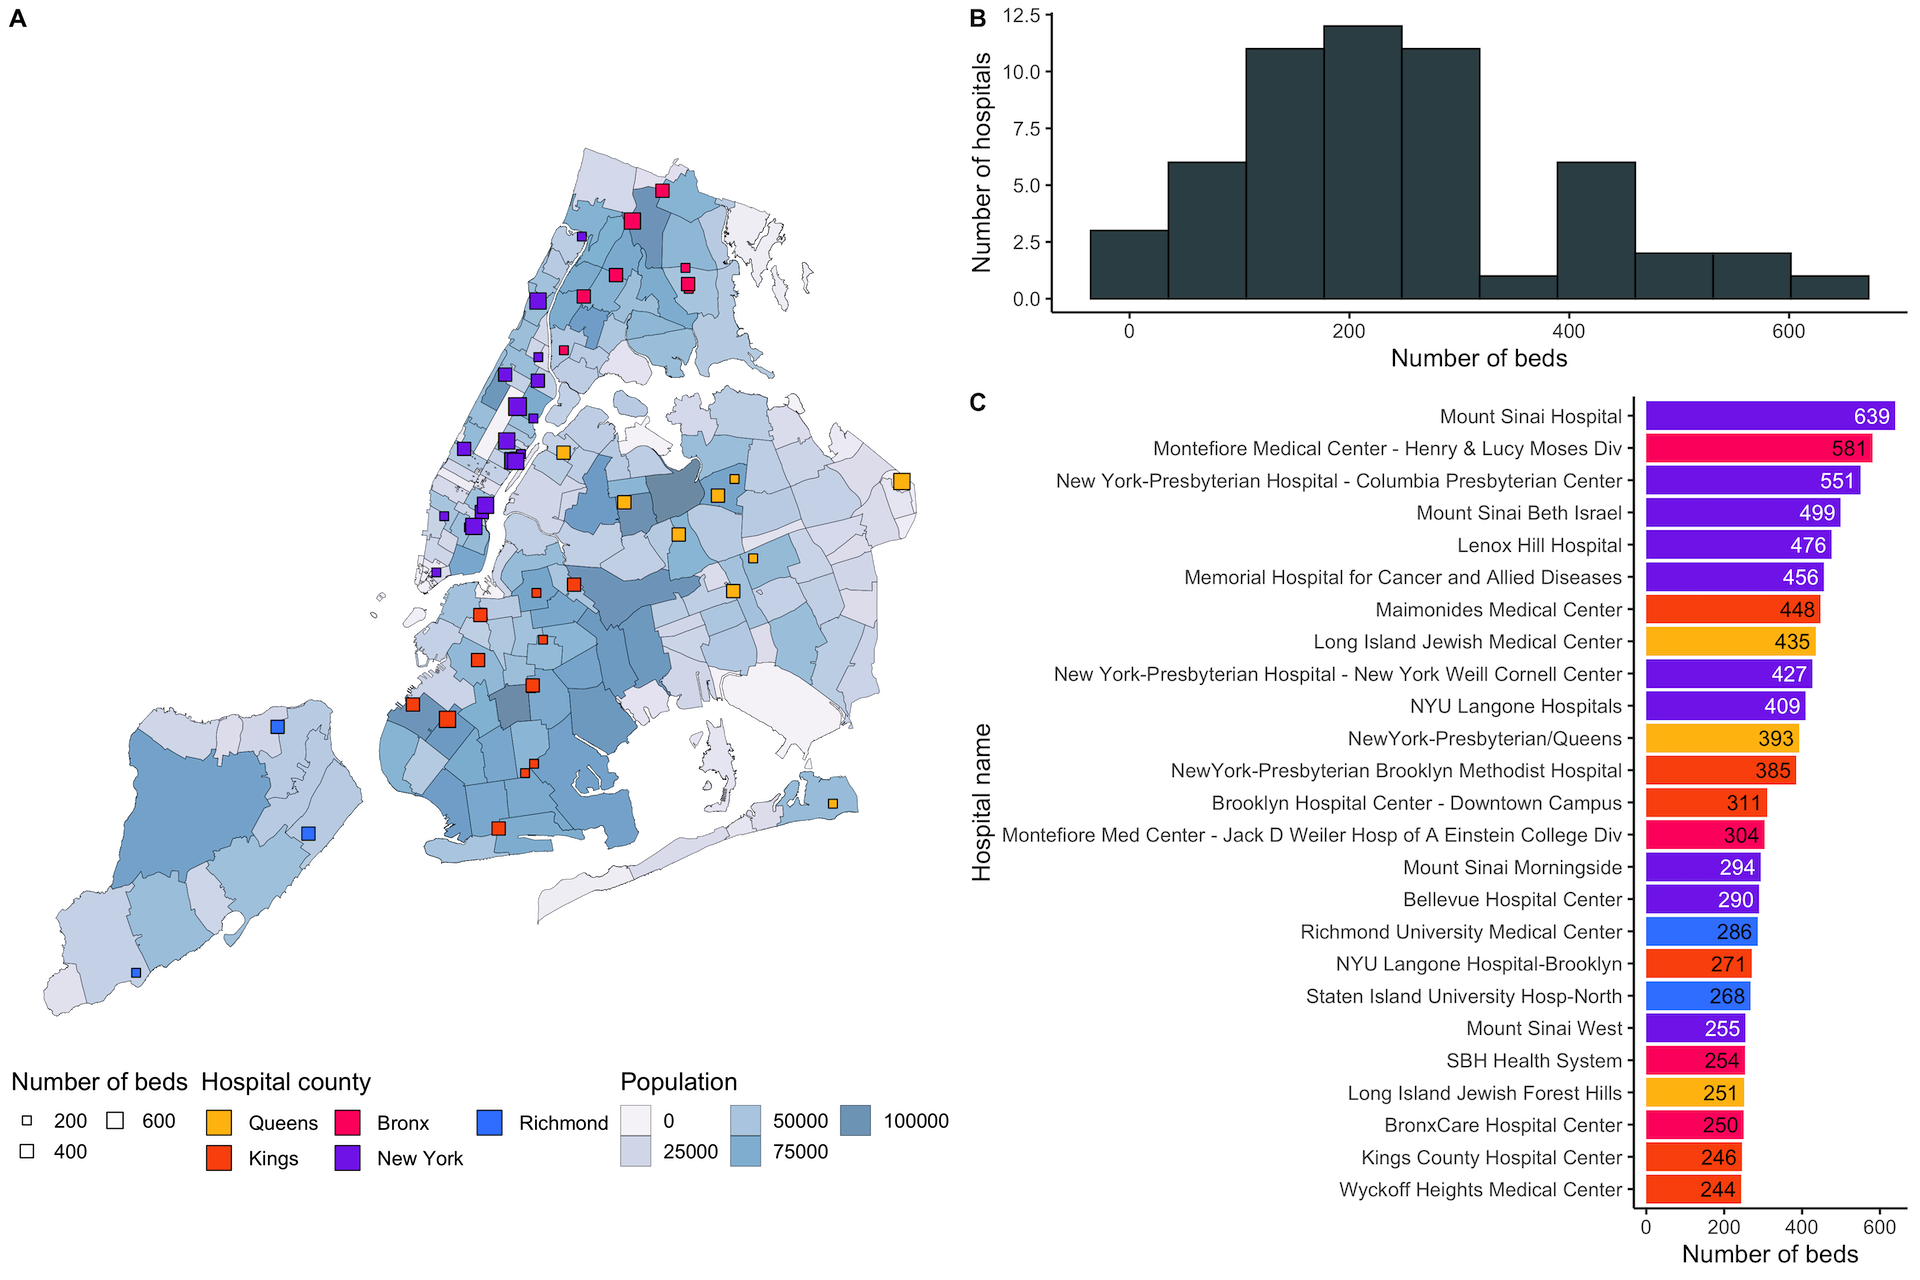
\includegraphics[width=0.9\textwidth]{images/routes/fig1.png}
    \centering
    \caption{
        \textbf{Patients routes in metropolitan France.} GPS routes with more than 5 patients are shown on map (A). Municipalities are colored by the average travel duration for patients with cancer. Patients who visit \ac{clcc} and \ac{chru} hospitals have longer travel durations (B); as well as patients who live in non-dense municipalities (C).
    }
    \label{fig:routes-duration-france}
\end{figure}

\begin{figure}[H]
    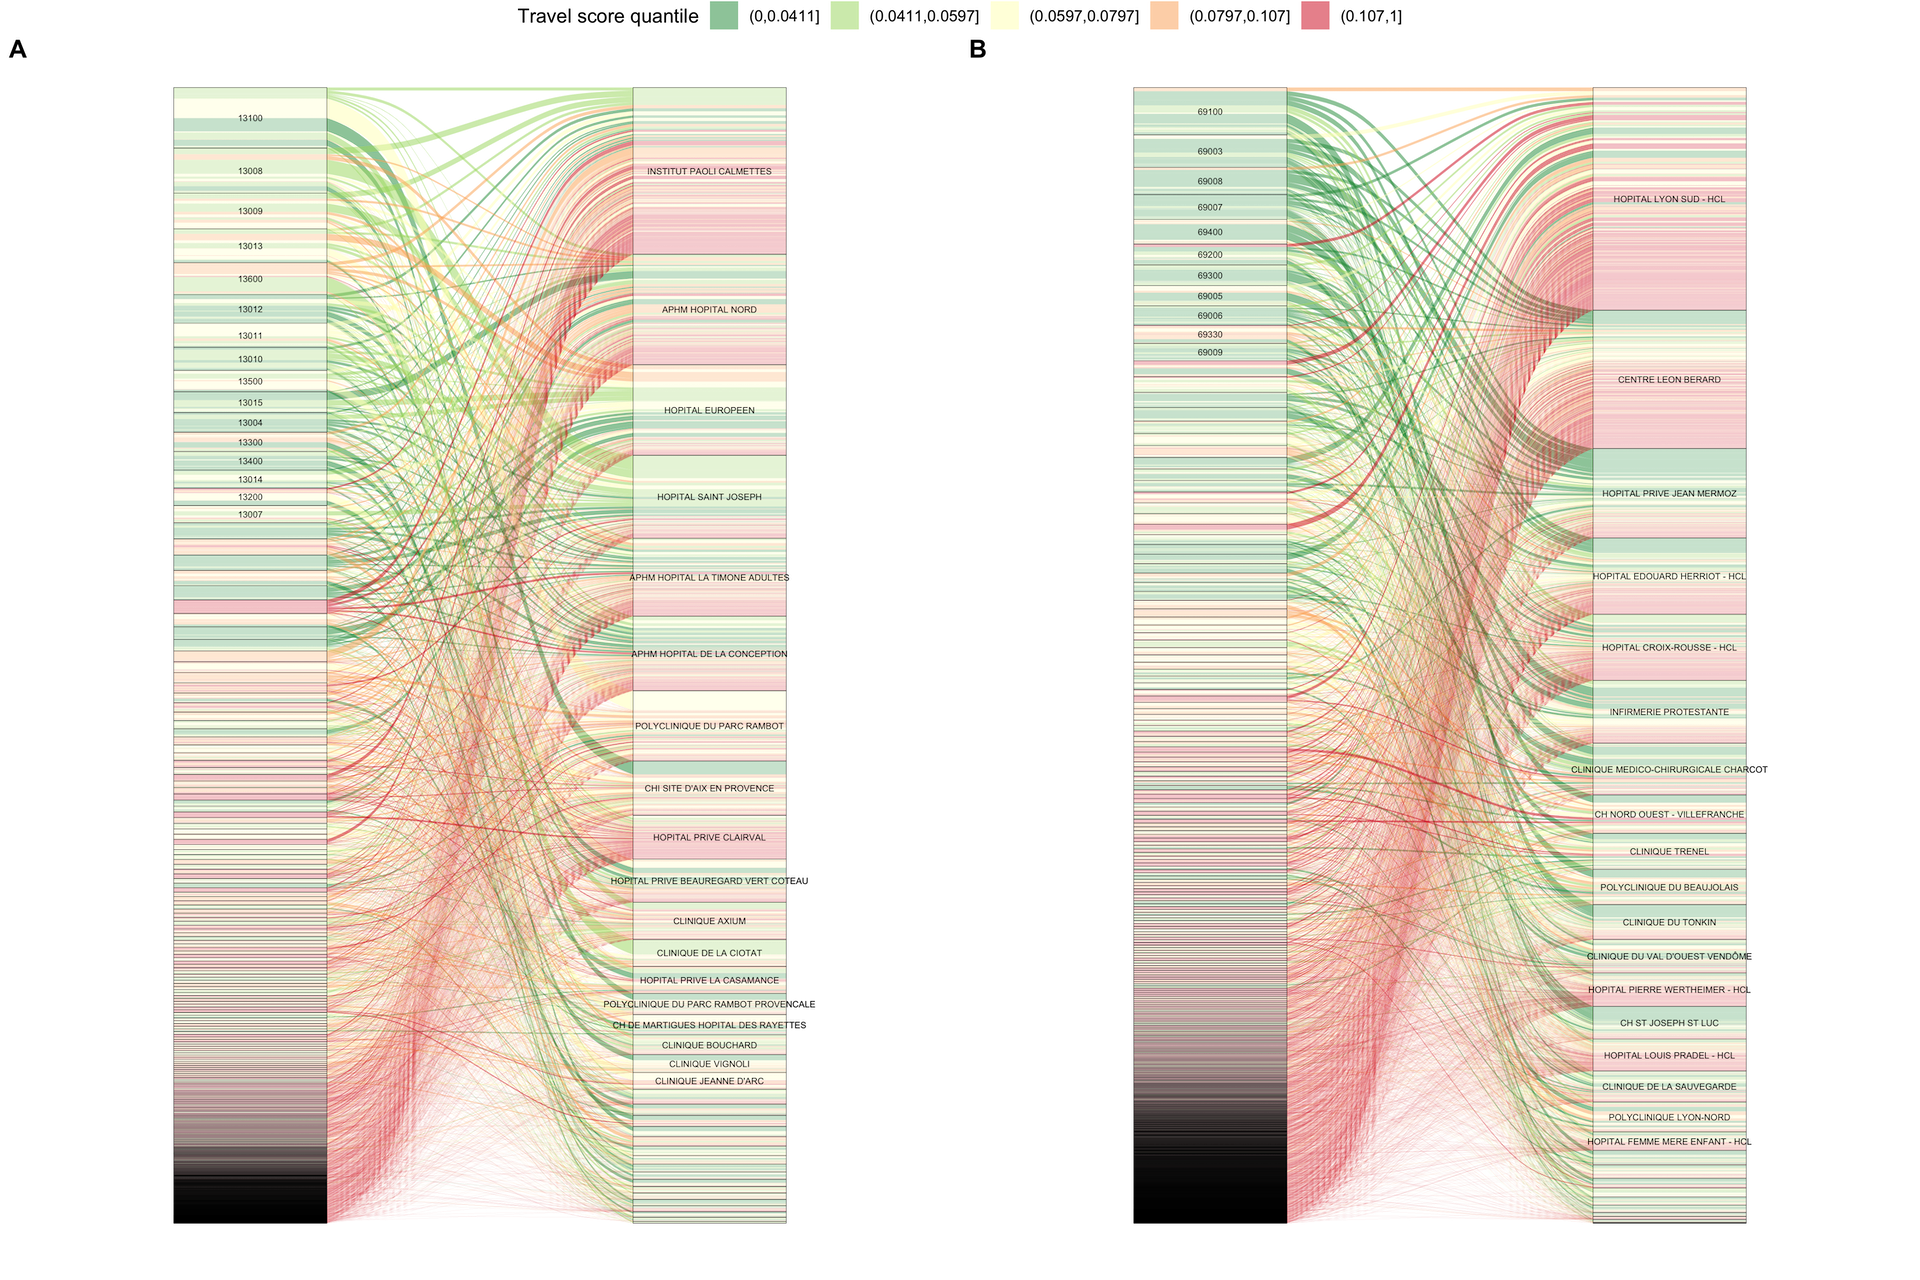
\includegraphics[width=0.9\textwidth]{images/routes/fig6.png}
    \centering
    \caption{
        \textbf{Distribution of patients traveling to care centers located in Bouches-du-Rhone department.} Municipalities are displayed on the right side of the alluvial plot, and care centers on the left side. Municipalities are sized by the number of residing patients. Care centers are sized by the number of treated patients. Flows represent patients travel and are sized by the number of patients traveling from a municipality to a care center. The flows are colored based on the travel score quantile. We can easily identify that the patients living in smaller municipalities are more likely to experience tedious travel. Larger care centers often receive patients from these smaller municipalities.
    }
    \label{fig:routes-alluvial-13}
\end{figure}

\begin{figure}[H]
    \includegraphics[width=0.9\textwidth]{images/routes/fig8.png}
    \centering
    \caption{
        \textbf{Patients travel, sized by number of travels, and colored by \ac{co2} emission.} We study the patients travel in Bourg-en-Bresse area, a sub-urban and rural area located in Auvergne-Rhone-Alpes region. Plot (A) displays the patients flows from municipalities on the right to care centers on the left. The flows are colored by the resulting \ac{co2} emissions. \ac{co2} emissions are calculated by multiplying the travel distance by the number of travels and the car average consumption. We can see that the higher \ac{co2} emissions are not issued by travels with lots of patients, but instead from travels with fewer patients but much longer drives. This is emphasized on plot (B), showing the \ac{co2} emissions resulting from patients living in Bourg en Bresse area. Indeed, the 42 travels to Hopital Lyon Sud emitted three times as much \ac{co2} than the 253 travels to Centre Hospitalier de Fleyriat.
    }
    \label{fig:routes-co2-01}
\end{figure}
